\chapter{Evaluation}

In this section, we first present an example of SMEIL used as an \gls{il}
followed by four simple examples implemented in SMEIL: A model watch using a
7-segment display, the core of a trading chip, a process for binning colors
based on intensity and finally an MD5 hash bruteforcer.

\todo{Motivate why these examples were picked in particular}

\section{SMEIL as an intermediate language}
\label{sec:smeilil}
We have made repeated references to the origins of SMEIL as a pure intermediate
language \gls{il} and described how and why the scope of the language was
widened to also include use as an independent implementation language. Despite
this, SMEIL is still very much intended to be also usable as an \gls{il}. As it
may be obvious at this point, the design, implementation and testing have mostly
focused on its use as a primary implementation language, with the \gls{il} angle
remaining in the background. Ideally, we would have a code generation backend
for C\# at this point, targeting SMEIL, since that is the most complete SME
implementation. However, this was not possible within the available time-frame
and in any case the implementation would need to be carried out by a third party
--- your present author is not sufficiently familiar with the C\# SME framework
to carry out the work himself. In the end, time had to be prioritized and the
time required to show a functioning proof-of-concept using SMEIL as an
intermediate language would have sacrificed significant parts of the
co-simulation interface.

It is never ideal to leave loose ends, so to show that using SMEIL as an
\gls{il} {\itshape can} be done we have adapted our previously implemented
Python to \gls{vhdl} compiler to generate SMEIL instead of generating VHDL
directly. This translation is not yet fully automated, but we explain how it
could be done here, and that doing it is in fact quite feasible.

As an example, we will show how the AllOps network is translated from PySME to
SMEIL. This implementation was first presented in~\cite{asheim2016vhdl} and is
used here unmodified. \todo{Show the translation}


\section{7-Segment Display}
\label{sec:7seg}
\begin{figure}%[tb]
\begin{minipage}{\linewidth}
  \centering
  \resizebox{.6\linewidth}{!}{
    \begin{tikzpicture}[font=\small,
      rep style/.style={rectangle,draw=black,text width=1.5cm,minimum
        size=1.5cm,align=center},
      proc style/.style={ellipse,draw=black,align=center,text
        width=1.5cm,minimum size=1.5cm,align=center},
      file style/.style={ellipse,draw=none,align=center,text
        width=1.5cm,minimum size=0.5cm,align=center},
      part/.pic={
        \node[] (m1) {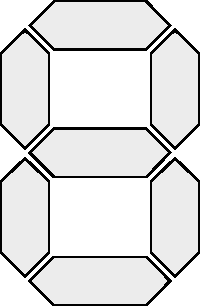
\includegraphics[width=.10\textwidth]{figures/7seg.pdf}};
        \node[left=0cm of m1] (m2) {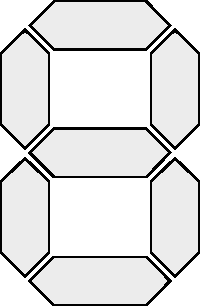
\includegraphics[width=.10\textwidth]{figures/7seg.pdf}};}
      ]

      \pic[local bounding box=hrs] {part};
      \node[below=2mm of hrs] (h2) {Hours};
      \pic[local bounding box=mins, right=30mm of hrs] {part};
      \node[below=2mm of mins] (m2) {Minutes};
      \pic[local bounding box=secs, right=30mm of mins] {part};
      \node[below=2mm of secs] (s2) {Seconds};

      \node[proc style, above=0.3cm of hrs] (dechrs) {Decoder};
      \node[proc style, above=0.3cm of mins] (decmins) {Decoder};
      \node[proc style, above=0.3cm of secs] (decsecs) {Decoder};

      \node[proc style, above=1cm of dechrs] (enchrs) {Encoder};
      \node[proc style, above=1cm of decmins] (encmins) {Encoder};
      \node[proc style, above=1cm of decsecs] (encsecs) {Encoder};
      
      \node[proc style, above=1cm of enchrs] (splithrs) {Calculate\\Hours};
      \node[proc style, above=1cm of encmins] (splitmins) {Calculate\\Minutes};
      \node[proc style, above=1cm of encsecs] (splitsecs) {Calculate\\Seconds};

      \draw[-{Latex[scale=1.6]}] (splithrs) edge (enchrs);
      \draw[-{Latex[scale=1.6]}] (splitmins) edge (encmins);
      \draw[-{Latex[scale=1.6]}] (splitsecs) edge (encsecs);

      \node[above=1cm of splitmins] (split) {};
      
      \node[proc style, above=2.5cm of split] (gen) {Timer};
      \draw[-] (gen) edge node [below left=0cm and 0cm of
      gen] {Seconds today} (split);

      \draw[-{Latex[scale=1.6]}] (split) edge (splithrs);
      \draw[-{Latex[scale=1.6]}] (split) edge (splitmins);
      \draw[-{Latex[scale=1.6]}] (split) edge (splitsecs);

      \draw[-{Latex[scale=1.6]}] (enchrs) edge (dechrs);
      \draw[-{Latex[scale=1.6]}] (encmins) edge (decmins);
      \draw[-{Latex[scale=1.6]}] (encsecs) edge (decsecs);

      \begin{scope}[on background layer]
        \node[draw=gray,inner sep=8pt,rounded corners=10pt,anchor=north
        west,fit=(enchrs)(encmins)(encsecs)(splithrs)(splitmins)(splitsecs)(gen),
        label={above}:Controller]
        (showhrs) {};
        \node[draw=gray,inner sep=8pt,rounded
        corners=10pt,anchor=north west,fit=(hrs)(dechrs)] (showhrs) {};
        \node[draw=gray,inner sep=8pt,rounded corners=10pt,anchor=north
        west,fit=(mins)(decmins)] (showmins) {}; \node[draw=gray,inner
        sep=8pt,rounded corners=10pt,anchor=north west,fit=(secs)(decsecs)]
        (showhrs) {};
      \end{scope}
    \end{tikzpicture}}
    \caption{Model digital watch using a 7-segment display. A timer keeps track
      of the number of seconds elapsed since midnight and several processes
      calculates and lights.
      \protect\footnote{7-segment digit rendering based on ``7
        segment display labeled''
        (\url{https://commons.wikimedia.org/wiki/File:7_segment_display_labeled.svg})
        by h2g2bob. CC BY-SA-3.0.}}
     %\protect\footnotemark}}
\label{fig:7seg}
\end{minipage}
  \end{figure}
    % \footnotetext{7-segment digit rendering based on ``7 segment display labeled''
    % (\url{https://commons.wikimedia.org/wiki/File:7_segment_display_labeled.svg})
    % by h2g2bob. CC BY-SA-3.0.}

  The first example, implements a model of an old-fashioned digital watch
  displaying the current time using 6 7-segment digits. The layout is depicted
  in \Cref{fig:7seg}. The timer process continuously increments a number,
  representing the number of seconds passed since turn-of-day, which is stored
  in the state of the process. For every cycle, the current number of seconds is
  emitted. This number is then broadcasted through a shared bus to a number of
  calculating processes which uses simple integer arithmetic to calculate the
  number of hours, minutes and seconds respectively. To better reflect an actual
  hardware implementation, encoder and decoder processes are inserted on the
  wire leading to the digit. They, respectively, encodes to and decodes from the
  bit-pattern used to light up parts of the 7-segment display.

  For representing the current time during simulation, the decoder processes are
  connected to a process which prints the current time in a readable format. The
  code for the process, with elisions, is shown in \Cref{fig:7segcode}.

  A real-world implementation of this design is simple to imagine: The timer
  process is replaced by an actual time-keeping device and the output of the
  encoder processes is connected directly to the 7-segment digits they
  drive. This network is implemented purely in SMEIL without depending on
  external processes for stimuli.

  \begin{figure}
    \centerfloat
\begin{lstlisting}[multicols=2, language=smeil]
proc timer ()
  bus elapsed {
    secs: uint;
  };
  const secs_per_day: uint = 86400;
  var cur: u17;
{
  cur = (cur + 1) % secs_per_day;
  elapsed.secs = cur;
}

proc hrs (in time)
  bus vals {
    d1: uint;
    d2: uint;
  };
  const secs_per_hr: uint = 3600;
  var cur: uint;
{
  cur = time.secs/secs_per_hr;
  vals.d1 = cur/10;
  vals.d2 = cur%10;
}

// [..]

proc encode (in inval)
  bus vals {
    d1: uint;
    d2: uint;
  };
  const digits: [10]uint =
    [0x7E, 0x30, 0x6D,
     0x79, 0x33, 0x5B,
     0x5F, 0x70, 0x7F,
     0x7B];
{
  vals.d1 = digits[inval.d1];
  vals.d2 = digits[inval.d2];
}

proc decode (in inval)
  bus vals {
    d1: uint;
    d2: uint;
  };
{
  switch inval.d1 {
    case 0 {vals.d1 = 0; }
    case 0x7E { vals.d1 = 0;}
    // [..]
    case 0x7B { vals.d1 = 9;}
    default { assert(false); }
  }
  //[..]
}

proc disp (in val1, in val2, in val3) {
  trace("{}{}:{}{}:{}{}",
    val1.d1, val1.d2,
    val2.d1, val2.d2,
    val3.d1, val3.d2);
}

network clock() {
  instance t  of timer();
  instance h  of hrs(t.elapsed);
  instance ench of encode(h.vals);
  instance dech of decode(ench.vals);
  // [..]
  instance _ of disp(dech.vals,
                     decm.vals,
                     decs.vals);
}
\end{lstlisting}
  \caption{Code of the 7-segment digital watch network.}
  \label{fig:7segcode}
\end{figure}  

\section{ColorBin}
\label{sec:colorbin}
\begin{figure}%[tb]
  \centering
  \resizebox{.7\linewidth}{!}{
    \begin{tikzpicture}[font=\small,
      rep style/.style={rectangle,draw=black,text width=1.5cm,minimum
        size=1.5cm,align=center},
      proc style/.style={ellipse,draw=black,align=center,text
        width=1.5cm,minimum size=1.5cm,align=center},
      file style/.style={ellipse,draw=none,align=center,text
        width=1.5cm,minimum size=0.5cm,align=center}
      ]
      \node[file style] (ims) {\ttfamily image1.jpg \\ \ttfamily image2.jpg \\ \ttfamily ...};
      
      \node[proc style, below right=-0.6cm and 2cm of ims] (gen) {Image \\ Reader};
      \node[proc style, below right=0cm and 3cm of gen] (collector) {Collector};
      \node[proc style, below=0.5cm of gen] (sink) {Sink};

      \draw[-{Latex[scale=1.6]}] (ims) edge (gen);
      \draw[-{Latex[scale=1.6]}] (gen) edge (collector);
      \draw[-{Latex[scale=1.6]}] (collector) edge (sink);
      
      \begin{scope}[on background layer]
        \node[draw=scopeborder,fill=scopebg,inner sep=10pt,rounded corners=10pt,anchor=north west,fit=(collector),label={above}:SMEIL] (SMEIL) {};
        \node[draw=scopeborder,fill=scopebg,inner sep=10pt,rounded corners=10pt,anchor=north west,fit=(gen)(sink),label={above}:PySME] (pysme) {};
      \end{scope}
    \end{tikzpicture}
  }
  \caption{The process network of ColorBin.}
  \label{net:colorbin}
\end{figure}


This network, named ColorBin (ported from the C\# version in
\cite{skovhede2017c++}), serially process the pixels in one or more images and
categorize their intensity as low (closer to black), medium and high (closer to
white). The generator reads images from the disk and separates each of their
pixels into RGB components. The input bus also has a boolean signal which is
true along with the last pixel of each image. That way, the collector process
(described next) can tell the images apart and reset its counters when a new
image begins. The collector process examines each pixel, placing it in one of
three intensity counters. When it receives the last-pixel token, it sends the
stored values of the intensity counters to the collector process which then
stores the pixel intensity counts for each image. The source code for the
collector process is shown. The SMEIL source code is shown in
\Cref{fig:collector}. The VHDL code generated for the process is shown in
\Cref{fig:vhdlc}. The mapping of names and structure from SMEIL to VHDL is
clearly seen. As is the immense verbosity of VHDL.

\begin{figure}

\begin{lstlisting}[language=smeil,multicols=2]
proc collector (in image_input)
  exposed bus bin_count_out {
    valid: bool;
    low: u32;
    med: u32;
    high: u32;
  };
// [..]
{
  if (image_input.valid) {
    color = ((image_input.R * 299) +
      (image_input.G * 587) +
      (image_input.B * 114)) / 1000;

    if (color > thresh_high) {
      counthigh = counthigh + 1;
    } elif (color > thresh_med) {
      countmed = countmed + 1;
    } else {
      countlow = countlow + 1;
    }
  }

  bin_count_out.low = countlow;
  bin_count_out.med = countmed;
  bin_count_out.high = counthigh;
  bin_count_out.valid =
    image_input.valid &&
    image_input.last_pixel;
}
\end{lstlisting}
  \caption{SMEIL source code for the collector process of the ColorBin network.}
  \label{fig:collector}
\end{figure}

\begin{figure}[hb!]
\centerfloat
  % \makebox[\textwidth][c]{
\begin{lstlisting}[language=vhdl]
entity collector is
  port (
    signal bin_count_out_valid: out boolean := false;
      -- [..]
  signal bin_count_out_high: out unsigned (31 downto 0) := to_unsigned(0, 32);
  signal image_input_valid: in boolean;
  -- [..]
  signal image_input_B: in unsigned (7 downto 0);
  signal clk: in std_logic;
  signal rst: in std_logic);
end entity collector;

architecture rtl of collector is
begin
  process (clk, rst) is
    constant thresh_high: integer := 200;
    -- [..]
    variable countlow: unsigned (31 downto 0) := to_unsigned(0, 32);
  begin
    if rst = '1' then
      bin_count_out_valid <= false;
      bin_count_out_low <= to_unsigned(0, 32);
      -- [..]
      countlow := to_unsigned(0, 32);
    elsif rising_edge(clk) then
      if image_input_valid then
        color := resize(((((((image_input_R *
                              to_unsigned(299, 10))) +
                            ((image_input_G * to_unsigned(587, 10)))) +
                           ((image_input_B * to_unsigned(114, 10))))) /
                         to_unsigned(1000, 10)),  color'length);
        if (color > thresh_high) then
          counthigh := resize((counthigh + to_unsigned(1, 32)),
                              counthigh'length);
        -- [...]
        end if;
      end if;
      bin_count_out_low <= resize(countlow, bin_count_out_low'length);
      -- [..]
\end{lstlisting}%}
  \caption{The VHDL code generated from the SMEIL code shown in
    \Cref{fig:collector}.}
  \label{fig:vhdlc}
\end{figure}

  
\section{High-frequency trading chip}
\begin{figure}%[tb]
  \centering
  \resizebox{.9\linewidth}{!}{
    \begin{tikzpicture}[font=\small,
      rep style/.style={rectangle,draw=black,text width=1.5cm,minimum
        size=1.5cm,align=center},
      proc style/.style={ellipse,draw=black,align=center,text
        width=1.5cm,minimum size=1.5cm,align=center},
      file style/.style={ellipse,draw=none,align=center,text
        width=1.5cm,minimum size=0.5cm,align=center},
      plot/.pic={
        \node[] (m1) {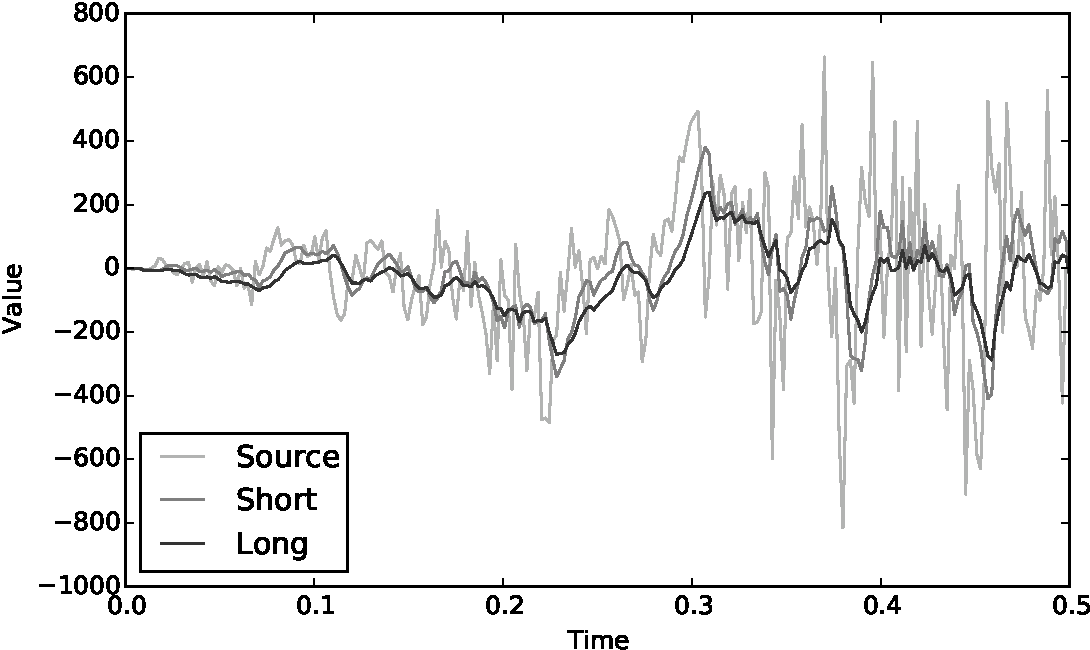
\includegraphics[width=.25\textwidth]{figures/ewma-plot.pdf}};
      }
      ]

      
      \node[proc style] (gen) {Data \\ Generator};
      \node[proc style, right=2cm of gen] (long) {Short Decay};
      \node[proc style, below=0.5cm of long] (short) {Long Decay};
      \node[proc style, below right=0cm and 1.5cm of long] (merge) {Merger};

      \node[proc style, below=0.5cm of gen] (sink) {Plotter};

      \pic[local bounding box=plot, above left=0cm and 2cm of sink] {plot};
      
      \draw[-{Latex[scale=1.6]}] (gen) edge (long);
      \draw[-{Latex[scale=1.6]}] (gen) edge (short);
      \draw[-{Latex[scale=1.6]}] (long) edge (merge);
      \draw[-{Latex[scale=1.6]}] (short) edge (merge);
      \draw[-{Latex[scale=1.6]}] (sink) edge (plot);

      % \draw[-{Latex[scale=1.6]}] (gen) edge (collector);

      \draw[-{Latex[scale=1.6]}] (merge) edge [bend left=50] (sink);
      
      \begin{scope}[on background layer]
        \node[draw=scopeborder,fill=scopebg,inner sep=10pt,rounded corners=10pt,anchor=north west,fit=(long)(short)(merge),label={above}:SMEIL] (SMEIL) {};
        \node[draw=scopeborder,fill=scopebg,inner sep=10pt,rounded corners=10pt,anchor=north west,fit=(gen)(sink),label={above}:PySME] (pysme) {};
      \end{scope}
    \end{tikzpicture}
  }
  \caption{The network of simpletrader.}
  \label{fig:simpletrade}
\end{figure}
We revisit an example from~\cite{asheim2016vhdl}. In high-frequency trading, a
split-second decision needs to be made whether to buy, or sell, a
stock. Reducing latency is paramount as you need to make transactions as fast as
possible. This problem is, therefore, an interesting target for custom hardware
as the intractable latencies induced by general-purpose hardware and
software-implemented decision-making logic are avoided. The real-time value of a
stock is passed through two calculator processes. Both calculate the exponential
moving average of a stock, one using long decay and the other using short
decay. The trading decision is based on detecting when the two averages
cross.~\cite{kablan2012use}

The network is shown in \Cref{fig:simpletrade} and the SMEIL source in
\Cref{fig:tradesrc}. The results of the two calculator processes described above
is passed through the merge process which combines the long and short averages
into a single bus. The core of the trader is written in SMEIL, while the
processes providing input stimuli and data collections is written in Python as a
PySME model. The input data is generated using a brownian
bridge~\cite{glasserman2003monte} which is a stochastic process commonly used as
a realistic model for simulating stock price developments. The results are
collected and visualized in a graph for easy verification.

In an actual trading chip, the data generator is replaced with actual stock
prices arriving through a network interface and the plot is replaced by market
transactions. Both the testing and verification processes leverage existing
Python libraries. The brownian bridge generator is implemented using NumPy while
the plot is made using matplotlib. Implementing these test processes in VHDL
would be a massive undertaking, With Python, it is quite simple.

\begin{figure}

\begin{lstlisting}[language=smeil, multicols=2]
sync proc calc (in data, const decay)
  bus result {
    val: int;
    valid: bool;
  };
  var prev: int;
  const sub: uint = 1;

{
  if (data.valid) {
    result.valid = true;
    prev = (data.val >> decay) +
      (prev >> decay) *
      ((1 << decay) - 1);
    result.val = prev;
  } elif (!data.valid) {
    result.val = prev;
  } else {
    result.valid = false;
  }
}

sync proc merge (in long,
                 in short, out res) {
  if (long.valid && short.valid) {
    res.valid = true;
    res.long = long.val;
    res.short = short.val;
  } else {
    res.valid = false;
  }
}

network ewma () {
  const decays: [2]uint = [2, 3];

  exposed bus stream {
    val: int;
    valid: bool;
  };

  exposed bus output {
    short: int;
    long: int;
    valid: bool;
  };

  instance short of calc 
      (data: stream, decay: decays[0]);
  instance long of calc
      (data: stream, decay: decays[1]);
  instance _ of merge
      (long: long.result,
       short: short.result,
       res: output);
}

\end{lstlisting}
  \caption{SMEIL source code for the trader core.}
  \label{fig:tradesrc}
   \end{figure}

\section{MD5 bruteforcer}
\begin{figure}%[tb]
  \centering
  \resizebox{.6\linewidth}{!}{
    \begin{tikzpicture}[font=\small,
      rep style/.style={rectangle,draw=black,text width=1.5cm,minimum
        size=1.5cm,align=center},
      proc style/.style={ellipse,draw=black,align=center,text
        width=1.5cm,minimum size=1.5cm,align=center},
      file style/.style={ellipse,draw=none,align=center,text
        width=1.5cm,minimum size=0.5cm,align=center}
      ]

      \node[proc style] (gen) {Input\\Generator};
      \node[proc style, right=1cm of gen] (calc) {MD5 Hasher};
      \node[proc style, right=1cm of calc] (verify) {Hash\\Verifier};

      \draw[-{Latex[scale=1.6]}] (gen) edge  (calc);
      \draw[-{Latex[scale=1.6]}] (calc) edge  (verify);

    \end{tikzpicture}}
  \caption{Structure of the MD5 bruteforcer network.}
  \label{fig:md5net}
\end{figure}

This example is a simplification of a bruteforcer of MD5-hashes developed to
showcase the performance of FPGAs in comparison with CPUs and GPGPUs for a
trivially parallelizable problem: Bruteforcing an MD5 hash. The layout of the
network is shown in \Cref{fig:md5net}. The generator iteratively emits all
combinations of 8 ASCII printable characters as a string. This string is then
passed to the hasher, calculating the MD5 sum of the string. In the verifier,
the calculated hash is compared to a pre-calculated hash of the input string
that we wish to find. The predictiveness of the input generator means that we
can ensure that the search terminates quickly by choosing a target string close
to the starting string. Hence, short runs can be chosen for testing and long
runs for benchmarking.

A complete implementation of this example exists for several targets: CPUs
parallelized with OpenMP, OpenCL for GPGPUs, Xilinx HLS and finally C\# SME.
Both the two latter implementations synthesizes and runs on FPGAs. A comparison
of these implementations showed that while GPUs were superior in raw
performance, the performance-per-watt ratio favored the FPGA significantly by
more than an order of magnitude. Furthermore, the SME version is significantly
more efficient than the Vivado HLS implementation, which relies on the
concurrency inference discussed in the introduction.

This example mainly serves to show an SMEIL implementation of an SME model which
has been synthesized to an FPGA. It also showcases an implementation a
non-trivial algorithm (MD5) in SMEIL. In particular, the MD5 algorithm relies
heavily on bit-shifting of 32-bit unsigned integers. Therefore, it depends on
the correctness of the integer overflow emulation of the \libsme{} simulator in
order to produce the expected result. The shortened source code of the SMEIL
process for calculating and MD5 hash is shown in \Cref{fig:smeilhash}. The
process receives the string that should be hashed through the bus passed as its
{\ttfamily input} parameter. The calculated hash is then sent on the {\ttfamily hashes} bus
which is read by the verification process.

\begin{figure}

\begin{lstlisting}[language=smeil, multicols=2]
proc md5(in input)
  bus hashes {
    h0: u32;
    h1: u32;
    h2: u32;
    h3: u32;

    w0: u32;
    w1: u32;
  };

  const r: [64]uint = [
    [...]
    6, 10, 15, 21, 6, 10]

  const kk: [64]uint = [
    0xd76aa478, 0xe8c7b756
    [..]
    0xf7537e82, 0xbd3af235
    ];

// Variable declarations omitted

{
  h0 = 0x67452301;
  // [..]

  w[0] = input.w0;
  w[1] = input.w1;
  w[2] = 128;
  w[14] = 64;

  a = h0;
  b = h1;
  c = h2;
  d = h3;

for i = 0 to 63 {
  if (i < 16) {
    f = (b & c) | ((~b) & d);
    g = i;
   // [..]
  } else {
    f = c ^ (b | (~d));
    g = (7 * i) % 16;
  }

  tmp = d;
  d = c;
  c = b;
  x = a + f + kk[i] + w[g];
  c2 = r[i];
  b = b + (((x) << (c2)) |
      ((x) >> (32 - (c2))));
  a = tmp;
}

h0 = h0 + a;
// [..]
h3 = h3 + d;

hashes.h0 = h0;
// [..]
hashes.h3 = h3;

hashes.w0 = w[0];
hashes.w1 = w[1];
}

\end{lstlisting}
  \caption{SMEIL source code for the MD5 hashing process.}
  \label{fig:smeilhash}

\end{figure}

\section{Performance}
The simulation performance of a hardware design tool is not essential as it does
not have an impact on the resulting implementation. Nevertheless, a slow
simulator can waste valuable developer time by inducing a long
develop-compile-test cycle.

The current implementation of SMEIL is not written with performance in mind and
leaves a lot of performance-related low-hanging fruits unpicked. Indeed, its
naïve interpreter makes repeated traversals of the SMEIL AST and the interface
between PySME and \libsme{} relies on the very general and inefficient
\textsc{libffi} library. Lastly, Python itself is not cherished for its
performance. It is therefore noteworthy that it still exceeds the performance of
the VHDL simulator GHDL, which generates native code before simulating. The VHDL
simulator of Xilinx Vivado, fails to complete the simulation due to memory
exhaustion.

Simulating 352,686 cycles of the ColorBin (\Cref{sec:colorbin}) network on an
Intel Core i7 6700HQ CPU at 2.60GHz, requires 47 seconds using GHDL but only 30
seconds using \libsme.


%%% Local Variables:
%%% mode: latex
%%% TeX-master: "../master"
%%% TeX-command-extra-options: "-enable-write18"
%%% End:
